% IEEE BSN 2026 — 4-page technical paper (references included)
% Compile from paper/:  pdflatex ieee_bsn2026.tex  (run twice)
\documentclass[conference]{IEEEtran}
\IEEEoverridecommandlockouts

\usepackage{cite}
\usepackage{amsmath,amssymb,amsfonts}
\usepackage{algorithmic}
\usepackage{graphicx}
\usepackage{textcomp}
\usepackage{xcolor}
\usepackage{booktabs}
\graphicspath{{figures/}}

\def\BibTeX{{\rm B\kern-.05em{\sc i\kern-.025em b}\kern-.08em
    T\kern-.1667em\lower.7ex\hbox{E}\kern-.125emX}}

\begin{document}

\title{Wearable EEG-Based Motor Imagery Classification for Real-Time Control of a Kinova Robotic Arm}

\author{
\IEEEauthorblockN{Shivansh Sharma, Parthan Olikkal, and Ramana Vinjamuri}
\IEEEauthorblockA{\textit{Vinjamuri Lab, Department of Computer Science and Electrical Engineering}\\
\textit{University of Maryland Baltimore County}\\
Baltimore, MD 21250, USA\\
Email: rvinjam1@umbc.edu}
}

\maketitle

\begin{abstract}
Brain-computer interfaces (BCIs) based on motor imagery (MI) can enable assistive control of robotic devices, but translating wearable electroencephalography (EEG) to reliable real-time actuation remains challenging due to inter-subject variability, limited channel count, and train-deploy preprocessing mismatches. We present an end-to-end MI-BCI system that acquires 8-channel EEG at 250\,Hz using the Unicorn Hybrid Black headset, decodes left- versus right-arm imagery with deep learning, and commands a Kinova Gen3 manipulator. A unified graphical interface orchestrates data collection, preprocessing, model training, and closed-loop control. We compare EEGNet, CTNet, and FBMSNet under subject-specific calibration (20 trials per class). Offline test accuracy ranged from 52.5\% to 90.0\% across five participants; EEGNet achieved the highest mean accuracy (69.6\%). Real-time inference uses 1\,s windows updated every 0.5\,s. An optional EEG-computer-vision hybrid mode modulates arm speed based on agreement between neural predictions and visual bar tracking.
\end{abstract}

\begin{IEEEkeywords}
Motor imagery, EEG, brain-computer interface, wearable sensing, deep learning, robotic arm
\end{IEEEkeywords}

\section{Introduction}
Motor imagery (MI) BCIs decode imagined limb movements from scalp EEG and have been applied to wheelchairs, prostheses, and robotic manipulators~\cite{pfurtscheller1997,pfurtscheller2006,ang2008}. Wearable EEG headsets now enable experiments outside traditional laboratories, but practical assistive systems require low-latency inference, deployment-aligned preprocessing, and integration with physical actuators~\cite{lotte2018}.

Convolutional architectures such as EEGNet~\cite{lawhern2018}, CTNet~\cite{ctnet2023}, and FBMSNet~\cite{fbmsnet2022} achieve strong performance on benchmark MI datasets. Less is known about their behavior on low-channel portable recordings coupled to closed-loop robotic control.

This work develops and evaluates a complete pipeline from wearable EEG acquisition to Kinova arm actuation. Contributions are: (i)~an integrated software framework for MI data collection, preprocessing, training, and real-time control; (ii)~subject-specific comparison of three deep EEG decoders on 8-channel, 250\,Hz recordings; (iii)~closed-loop inference at 2\,Hz (0.5\,s update interval) on 1\,s windows; and (iv)~an optional EEG-vision fusion mode for speed modulation.

\section{Methods}

\subsection{Participants and Experimental Protocol}
Five healthy participants (Subjects S1--S4 and S10; ages 19--35) completed a two-class MI session after providing informed consent. Each performed:
\begin{itemize}
    \item \textbf{Class 1:} imagine right-arm movement (``Up / Right Arm'')
    \item \textbf{Class 2:} imagine left-arm movement (``Down / Left Arm'')
\end{itemize}
Each trial comprised: 1\,s baseline, 2\,s instruction, and 5\,s MI/stimulus. A 20\,s stabilization period preceded recorded trials. Twenty randomized trials per class were collected per subject.

\subsection{EEG Acquisition}
EEG was recorded with the Unicorn Hybrid Black (g.tec) at 250\,Hz using eight scalp channels (Ch1--Ch8). A custom PyQt5 application tagged each sample with \texttt{trial\_index}, \texttt{class\_label}, and \texttt{phase} (baseline, instruction, stimulus). Data were stored as CSV files.

\subsection{Preprocessing and Training}
Raw trials were bandpass filtered (Butterworth, zero-phase, 4--40\,Hz). MI segments were fixed to 1250 samples (5\,s). An 80/20 stratified trial-level train/test split (seed 42) prevented window leakage.

\textbf{EEGNet/CTNet:} 1\,s windows (250 samples), 50\% training overlap, per-window z-score normalization aligned with real-time inference. Baseline normalization was disabled to match streaming deployment.

\textbf{FBMSNet:} Nine sub-bands (4--8\,Hz through 36--40\,Hz), 248-sample windows, per-band normalization.

Models were trained subject-specifically. EEGNet used Adam ($\text{lr}=10^{-4}$), class-weighted cross-entropy, ReduceLROnPlateau, and early stopping (patience 100).

\subsection{Real-Time Closed-Loop Control}
A rolling buffer holds 250 samples (1\,s). Every 0.5\,s the system bandpass filters (4--40\,Hz), z-score normalizes per channel, runs inference, and maps the predicted class to predefined Kinova joint configurations (class 0 = right, class 1 = left).

\textbf{Hybrid mode:} A camera tracks a colored bar. When the EEG-predicted direction matches the visually tracked direction, the arm moves at full speed; on mismatch, speed is reduced by 50\%.

\section{Results}

\subsection{Offline Classification}
Table~\ref{tab:accuracy} reports offline test accuracy from the latest subject-specific run per model.

\begin{table}[htbp]
\caption{Offline test accuracy (\%) per subject and model (latest run).}
\label{tab:accuracy}
\begin{center}
\begin{tabular}{lccc}
\toprule
\textbf{Subject} & \textbf{EEGNet} & \textbf{CTNet} & \textbf{FBMSNet} \\
\midrule
S1  & 90.0 & ---  & ---  \\
S2  & 63.1 & 53.8 & 60.0 \\
S3  & 72.8 & 46.4 & 54.5 \\
S4  & 52.5 & 48.8 & 53.8 \\
S10 & 69.6 & 51.8 & 59.3 \\
\midrule
Mean & \textbf{69.6} & 50.2 & 56.9 \\
\bottomrule
\end{tabular}
\end{center}
\end{table}

EEGNet achieved the highest accuracy for all five subjects with available runs (mean 69.6\%). Performance was highly subject-dependent: S1 reached 90.0\% while S4 remained near chance (52.5\%). CTNet and FBMSNet were near or below 55\% on average across the four subjects with complete model coverage.

\subsection{System Integration}
Fig.~\ref{fig:system} summarizes the end-to-end architecture. The unified GUI links data collection, notebook-based preprocessing, training, and deployment. Real-time controllers load subject-specific checkpoints and stream predictions at 2\,Hz.

\begin{figure}[htbp]
\centerline{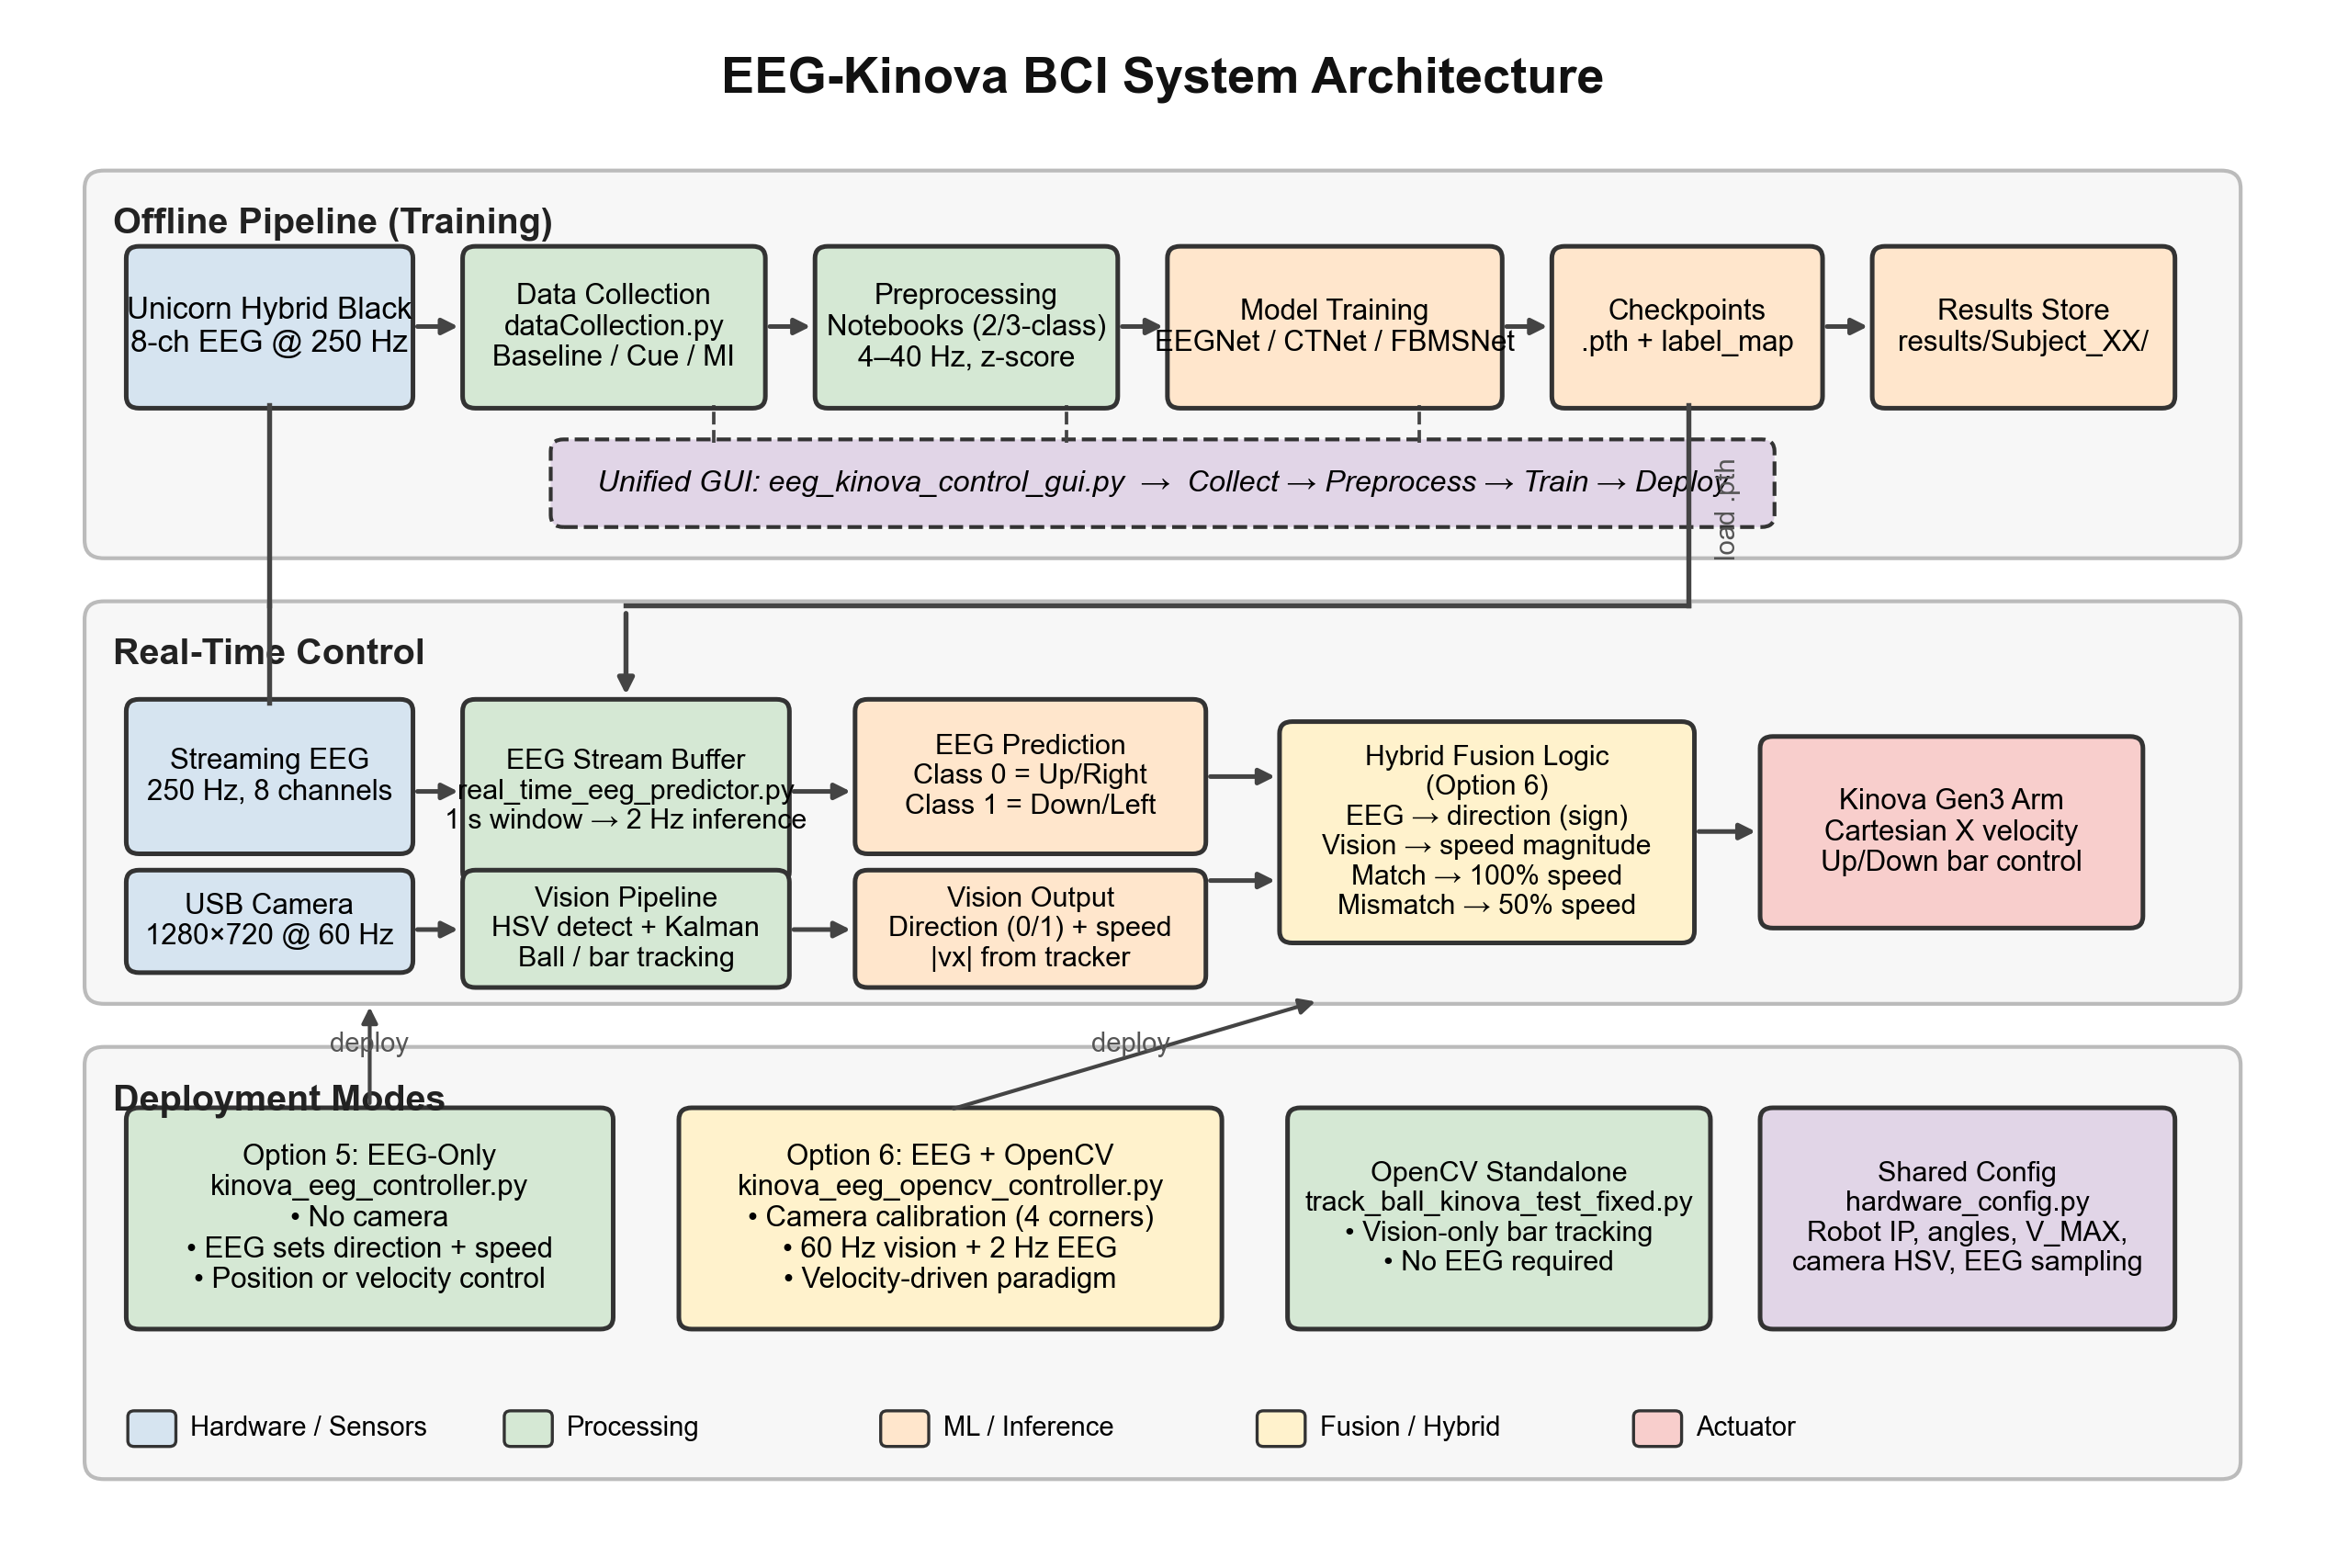
\includegraphics[width=\columnwidth]{fig1_system_architecture.png}}
\caption{End-to-end wearable EEG pipeline for motor-imagery decoding and Kinova robotic arm control. Offline training uses subject-specific models; real-time control applies 1\,s windows updated every 0.5\,s. Optional EEG-vision fusion modulates arm speed.}
\label{fig:system}
\end{figure}

\section{Discussion}
Results demonstrate feasibility of portable 8-channel EEG-driven robotic control with subject-specific deep models. The large inter-subject spread (52.5\%--90.0\%) is consistent with known BCI illiteracy effects~\cite{lotte2018} and the limited training set (32 trials per subject after splitting). Window augmentation increases sample count but not independent trials, which may inflate offline metrics relative to trial-grouped evaluation.

A critical deployment lesson was preprocessing alignment: offline training must match real-time filtering (4--40\,Hz), window length (250 samples for EEGNet/CTNet), and normalization (per-window z-score without baseline correction). Inconsistent channel indexing or normalization caused model collapse in development runs.

Limitations include: small cohort ($N{=}5$), no quantitative real-time success-rate metrics yet reported, and simplified FBMSNet real-time inference (single-band replication rather than full nine-band filter bank). Future work will add trial-grouped cross-validation, majority-vote smoothing, larger per-subject datasets, and quantitative hybrid-mode control metrics.

\section{Conclusion}
We presented a wearable EEG-based MI system for real-time Kinova robotic arm control, integrating acquisition, deep learning, and closed-loop actuation. EEGNet outperformed CTNet and FBMSNet on average (69.6\% vs.\ 50.2\% and 56.9\%), with peak subject-specific accuracy of 90.0\%. The framework highlights both the promise of portable EEG-driven assistive robotics and the need for subject-specific calibration and deployment-aligned preprocessing.

\section*{Acknowledgment}
The authors thank the Vinjamuri Lab for support. [Add funding agency acknowledgment here if applicable.]

\section*{References}

\begin{thebibliography}{10}

\bibitem{pfurtscheller1997}
G.~Pfurtscheller and F.~H.~Lopes da Silva, ``Event-related EEG/MEG synchronization and desynchronization: basic principles,'' \emph{Clin. Neurophysiol.}, vol.~110, no.~11, pp.~1842--1857, 1999.

\bibitem{pfurtscheller2006}
G.~Pfurtscheller, C.~Brunner, A.~Schl{\"o}gl, and F.~H.~Lopes da Silva, ``Mu rhythm (de)synchronization and EEG single-trial classification of different motor imagery tasks,'' \emph{NeuroImage}, vol.~31, no.~1, pp.~153--159, 2006.

\bibitem{ang2008}
K.~K.~Ang, Z.~Chin, C.~Wang, C.~Guan, and H.~Zhang, ``Filter bank common spatial pattern algorithm on BCI competition IV datasets 2a and 2b,'' \emph{Front. Neurosci.}, vol.~6, p.~39, 2012.

\bibitem{lotte2018}
F.~Lotte et al., ``A review of classification algorithms for EEG-based brain--computer interfaces: a 10 year update,'' \emph{J. Neural Eng.}, vol.~15, no.~3, p.~031005, 2018.

\bibitem{lawhern2018}
V.~J.~Lawhern, A.~J.~Solon, N.~R.~Waytowich, S.~M.~Gordon, C.~P.~Hung, and B.~J.~Lance, ``EEGNet: a compact convolutional neural network for EEG-based brain--computer interfaces,'' \emph{J. Neural Eng.}, vol.~15, no.~5, p.~056013, 2018.

\bibitem{ctnet2023}
[Add full CTNet citation from your thesis bibliography]

\bibitem{fbmsnet2022}
[Add full FBMSNet citation from FBMSNet repository paper]

\bibitem{blankertz2010}
B.~Blankertz et al., ``The Berlin Brain--Computer Interface: non-medical uses of BCI technology,'' \emph{Front. Neurosci.}, vol.~4, p.~198, 2010.

\bibitem{schirrmeister2017}
R.~T.~Schirrmeister et al., ``Deep learning with convolutional neural networks for EEG decoding and visualization,'' \emph{Hum. Brain Mapp.}, vol.~38, no.~11, pp.~5391--5420, 2017.

\bibitem{unicorn}
g.tec medical engineering GmbH, ``Unicorn Hybrid Black,'' product documentation, accessed 2026.

\end{thebibliography}

\end{document}
